% ᾶῖῶῆῦ  
% ἀἰὐἐὀὠἠ 
% ὰὲὶὸὺὼὴ 
% ἁἱὑὁὡἡῥ
% άέίόύήώΆΉ
% ἂἒὒἲὂὢἢὒἚἊ
% ἃἳὓὃἣὣἓἋἛ
% ἄἔἴὄὔὤἤἌἬ
% ἅἕἵὅὕὥἥἍἭ
% ἆὦἶἦὖἯἏὯἇὧἷἧὗἯἏὯ 

% ᾳῃῳ
% ᾱῑῡ
% ᾀᾐᾠ
% ᾰῐῠ
% ᾂᾒᾢ
% ϊ ϋ
% ᾄᾔᾤ
% ΰ ΐ
% ᾆᾖᾦ
% ᾲῂῲ
% ᾴῄῴ
% ᾷῇῷ


\documentclass[nols]{tufte-handout}

%\geometry{showframe} % display margins for debugging page layout

\usepackage{fontspec}
\usepackage{ifxetex}
\setmainfont[Path=./fonts/palatino-linotype/, ItalicFont=palai.ttf, BoldFont=palab.ttf]{pala.ttf}


% \defaultfontfeatures{Mapping=tex-text}
% \setromanfont[Path=./fonts/TeX-Gyre-Schola/,Mapping=tex-text]{TeX Gyre Schola}
% \setsansfont[Path=./fonts/TeX-Gyre-Heros/,Scale=MatchLowercase,Mapping=tex-text]{TeX Gyre Heros}
% \setmonofont[Path=./fonts/TeX-Gyre-Cursor/,Scale=MatchLowercase]{TeX Gyre Cursor}

\usepackage{lipsum}
\usepackage{url}
\usepackage{longtable}


\usepackage{graphicx} % allow embedded images
  \setkeys{Gin}{width=\linewidth,totalheight=\textheight,keepaspectratio}
  \graphicspath{{graphics/}} % set of paths to search for images
\usepackage{amsmath}  % extended mathematics
\usepackage{booktabs} % book-quality tables
\usepackage{units}    % non-stacked fractions and better unit spacing
\usepackage{multicol} % multiple column layout facilities
\usepackage{lipsum}   % filler text
\usepackage{fancyvrb} % extended verbatim environments
  \fvset{fontsize=\normalsize}% default font size for fancy-verbatim environments

% Standardize command font styles and environments
\newcommand{\doccmd}[1]{\texttt{\textbackslash#1}}% command name -- adds backslash automatically
\newcommand{\docopt}[1]{\ensuremath{\langle}\textrm{\textit{#1}}\ensuremath{\rangle}}% optional command argument
\newcommand{\docarg}[1]{\textrm{\textit{#1}}}% (required) command argument
\newcommand{\docenv}[1]{\textsf{#1}}% environment name
\newcommand{\docpkg}[1]{\texttt{#1}}% package name
\newcommand{\doccls}[1]{\texttt{#1}}% document class name
\newcommand{\docclsopt}[1]{\texttt{#1}}% document class option name
\newenvironment{docspec}{\begin{quote}\noindent}{\end{quote}}% command specification environment

% concetti morfosintattici
\usepackage{xspace} 
\newcommand{\noun}{\textsc{sostantivo}\xspace}
\newcommand{\nouns}{\textsc{sostantivi}\xspace}
\newcommand{\adject}{\textsc{aggettivo}\xspace}
\newcommand{\adjects}{\textsc{aggettivi}\xspace}
\newcommand{\gnumber}{\textsc{numero}\xspace}
\newcommand{\gnumbers}{\textsc{numeri}\xspace}
\newcommand{\gender}{\textsc{genere}\xspace}
\newcommand{\genders}{\textsc{generi}\xspace}
\newcommand{\gcase}{\textsc{caso}\xspace}
\newcommand{\gcases}{\textsc{casi}\xspace}
\newcommand{\tense}{\textsc{tempo}\xspace}
\newcommand{\mood}{\textsc{modo}\xspace}
\newcommand{\gverb}{\textsc{verbo}\xspace}
\newcommand{\gverbs}{\textsc{verbi}\xspace}
\newcommand{\adjective}{\textsc{aggettivo}\xspace}
\newcommand{\nom}{\textsc{nom}\xspace}
\newcommand{\gen}{\textsc{gen}\xspace}
\newcommand{\dat}{\textsc{dat}\xspace}
\newcommand{\acc}{\textsc{acc}\xspace}
\newcommand{\voc}{\textsc{voc}\xspace}
\newcommand{\gexit}{\textsc{uscita}\xspace}
\newcommand{\gexits}{\textsc{uscite}\xspace}
\newcommand{\declinazione}{\textsc{declinazione}\xspace}
\newcommand{\masc}{\textsc{maschile}\xspace}
\newcommand{\femm}{\textsc{femminile}\xspace}
\newcommand{\neut}{\textsc{neutro}\xspace}

\newcommand{\indic}{\textsc{indicativo}\xspace}
\newcommand{\imper}{\textsc{imperativo}\xspace}
\newcommand{\gcong}{\textsc{congiuntivo}\xspace}
\newcommand{\ott}{\textsc{ottativo}\xspace}
\newcommand{\partic}{\textsc{participio}\xspace}
\newcommand{\infin}{\textsc{infinito}\xspace}

\newcommand{\pres}{\textsc{presente}\xspace}
\newcommand{\imperf}{\textsc{imperfetto}\xspace}
\newcommand{\aor}{\textsc{aoristo}\xspace}
\newcommand{\fut}{\textsc{futuro}\xspace}

\newcommand{\sing}{\textsc{singolare}\xspace}
\newcommand{\plur}{\textsc{plurale}\xspace}
\newcommand{\dual}{\textsc{duale}\xspace}


% italianitudini
\renewcommand{\figurename}{Figura}
\renewcommand{\tablename}{Tabella}
\renewcommand{\contentsname}{Indice}

% fix per un qualche problema
\ifxetex
  \newcommand{\textls}[2][5]{%
    \begingroup\addfontfeatures{LetterSpace=#1}#2\endgroup
  }
  \renewcommand{\allcapsspacing}[1]{\textls[15]{#1}}
  \renewcommand{\smallcapsspacing}[1]{\textls[10]{#1}}
  \renewcommand{\allcaps}[1]{\textls[15]{\MakeTextUppercase{#1}}}
  \renewcommand{\smallcaps}[1]{\smallcapsspacing{\scshape\MakeTextLowercase{#1}}}
  \renewcommand{\textsc}[1]{\smallcapsspacing{\textsmallcaps{#1}}}
\fi

\title{A Greek Primer. Introduzione al Greco Antico \newline Lezione IV - Nomi: neutri della declinazione in O.}

\author[gpciceri]{a cura di Milagathòs: Milo's help to enjoy humanities\marginnote{\url{http://www.milagathos.com}}
}

\date{29 Dicembre 2016} % without \date command, current date is supplied





\begin{document}

\maketitle% this prints the handout title, author, and date

\begin{marginfigure}[-2.5cm]
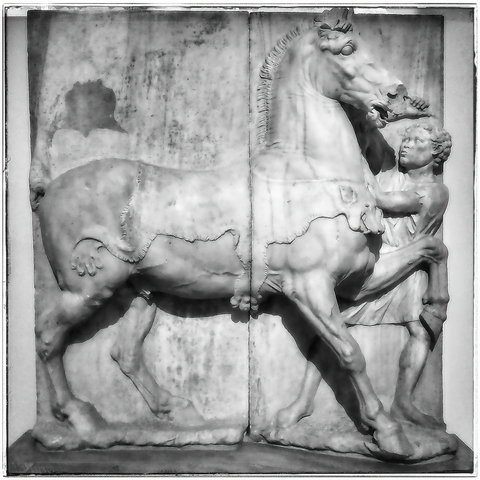
\includegraphics{smallthumb-lesson_I.jpeg}
\setfloatalignment{b}
\end{marginfigure}


\begin{abstract}
\noindent
Queste lezioni si articolano in \textsc{elementi grammaticali}, 
espressi sommariamente, seguiti da \textsc{vocabolari} per il lessico di base 
e da \textsc{frasi da tradurre} dal greco e in greco. 
\
L'approccio è quello del testo-laboratorio di morfosintassi: 
si presenta punto per punto - riprendendone la numerazione - 
l'esposizione di Gleason\cite{gleason1903}.\\
\bigskip
\noindent
Lezione IV: i nomi di genere neutro della declinazione in O,
considerazioni sugli accenti dei nomi, vocabolario, esercizi.
\end{abstract}

%\printclassoptions

\newthought{66. Modelli}

\begin{fullwidth}
\begin{table}[!htbp]
  \centering
  \begin{tabular}{l l c l l l l}
    %\toprule
	\multicolumn{7}{c}{\textsc{parole guida}} \\
	\multicolumn{2}{c}{\textbf{δῶρον,}}              & \textsc{nome latino}    & \textbf{πεδίον},               & \multicolumn{3}{c}{\textbf{τὸ καλὸν ἱμάτιον},} \\
	\multicolumn{2}{c}{\textit{dono,} \textsc{n.}} & \textsc{corrispondente} & \textit{pianura,} \textsc{n.}  & \multicolumn{3}{c}{\textit{il bel mantello}} \\
   
	\multicolumn{7}{c}{\textsc{singolare}} \\
    \textsc{n.} & \textbf{δῶρον} & \textit{donum} & \textbf{πεδίον} & \textbf{τὸ}   & \textbf{καλὸν} & \textbf{ἱμάτιον}  \\
    \textsc{g.} & \textbf{δώρου} & \textit{doni}  & \textbf{πεδίου} & \textbf{τοῦ} & \textbf{καλοῦ} & \textbf{ἱματίου}  \\
    \textsc{d.} & \textbf{δώρῳ}  & \textit{dono}  & \textbf{πεδίῳ}  & \textbf{τῷ}  & \textbf{καλῷ}  & \textbf{ἱματίῳ}  \\
	\textsc{a.} & \textbf{δῶρον} & \textit{donum} & \textbf{πεδίον} & \textbf{τὸ} & \textbf{καλὸν} & \textbf{ἱμάτιον}  \\
	\textsc{v.} & \textbf{δῶρον}  & \textit{donum}  & \textbf{πεδίον}  & \textemdash  & \textbf{καλὸν}  & \textbf{ἱμάτιον}  \\
	
	\multicolumn{7}{c}{\textsc{plurale}} \\
	\textsc{n.} & \textbf{δῶρα}  & \textit{dona}    & \textbf{πεδία}  & \textbf{τὰ}   & \textbf{καλὰ}  & \textbf{ἱμάτα}  \\
    \textsc{g.} & \textbf{δῶρων}  & \textit{donorum} & \textbf{πεδίων}  & \textbf{τῶν}  & \textbf{καλῶν}  & \textbf{ἱματίων}  \\
    \textsc{d.} & \textbf{δώροις} & \textit{donis}   & \textbf{πεδίοις} & \textbf{τοὶς} & \textbf{καλοῖς} & \textbf{ἱματίοις}  \\
	\textsc{a.} & \textbf{δῶρα} & \textit{dona}   & \textbf{πεδία} & \textbf{τὰ} & \textbf{καλὰ} & \textbf{ἱμάτια}  \\
	\textsc{v.} & \textbf{δῶρα}  & \textit{dona}   & \textbf{πεδία}  & \textemdash   & \textbf{καλὰ}  & \textbf{ἱμάτια}  \\
    %\bottomrule
  \end{tabular}
  \label{tab:normaltab}
  %\zsavepos{pos:normaltab}
\end{table}
\end{fullwidth}

\newthought{Osservazioni}
\begin{itemize}
\item[\textsc{1.}] In \textbf{πεδίον} e \textbf{δῶρον}, come in tutti i nomi neutri, i casi diretti (nominativo, accusativo e vocativo) sono uguali, e al plurale terminano in \textbf{α.} Confronta con il latino \textbf{donum}.  
\item[\textsc{2. Esercizio}] Declina in questo modo anche \textbf{χωρίον,} \textit{luogo, posto} e \textbf{ἱερόν,} \textit{tempio}.
\end{itemize}

\newthought{67. Accento dei nomi.} L'accento del nominativo singolare, per ogni parola nuova, deve essere imparato per osservazione diretta.

\newthought{68.} gli altri casi mantengono l'accento del nominativo se l'ultima sillaba lo permette (32), come in \textbf{λόγος, λόγου}; ma \textbf{δῶρον, δώρου}.

\newthought{69.} Le parole ossitone\sidenote{Una parola si dice \textit{ossìtona} se l'accento, acuto, cade sulla sua ultima sillaba.} (al nominativo singolare) presentano accento circonflesso 
su genitivo e dativo per tutti i numeri, come in \textbf{θεός,} \textit{il dio}, \textbf{θεοῦ,} \textit{del dio}.

\newthought{70. Vocabolario}

\begin{multicols}{2}
    \noindent \hangindent=1em \textbf{δῶρον,} \textit{dono}.  \\
    \noindent \hangindent=1em \textbf{ἱερόν,} \textit{tempio}.  \\
    \noindent \hangindent=1em \textbf{ἱμάτιον,} \textit{mantello}.  \\
    \noindent \hangindent=1em \textbf{πεδίον,} \textit{piana}.  \\
    \noindent \hangindent=1em \textbf{τέκνον,} \textit{bambino}.  \\
    \noindent \hangindent=1em \textbf{χωρίον,} \textit{posto, luogo}.  \\
    \noindent \hangindent=1em \textbf{κακός, κακόν,} \textit{cattivo, codardo}.  \\
    \noindent \hangindent=1em \textbf{εὑρίσκω,} fut. \textbf{εὑρήσω,} \textit{trovare, scoprire}.  \\
    \noindent \hangindent=1em \textbf{γάρ,} cong. postpositiva, \textit{infatti}. In latino \textit{enim}.   \\
    \noindent \hangindent=1em \textbf{ἐν,} \textit{in}, prep. con dat.  \\
    \noindent \hangindent=1em \textbf{ἐξ,} \textit{da, fuori da}, prep. con gen. (\textbf{ἐκ} prima di una consonante). \\ 
\end{multicols}

\newthought{71. Traduci:}
\textsc{1.}~ἱερον καλὸν ἦν ἐν τῷ πεδίῷ. \quad
\textsc{2.}~οὐκ ἄξουσι δὲ τὰ τέκνα εἰς τὸ ἱερόν. \quad
\textsc{3.}~ἐκ τοῦ χωρίον φεύγουσιν \quad
\sidenote{Una \textbf{ν}, detta \textbf{ν} mobile (\textbf{ν} \textit{efelcistico}), è aggiunta alla terza persona singolare che termina in \textbf{ε} 
e a tutte le parole che teminano in \textbf{σι}, se la parola successiva inizia con una vocale o se siamo alla fine di una frase.} οἱ ἵπποι. \quad
\textsc{4.}~οἱ δὲ τοῦ δούλου υἱοὶ ἔχουσι κακὰ ἱμάτια. \quad
\textsc{5.}~πέμψει γὰρ δῶρα τῷ ἀγαθῷ ἀνθρώπῳ. \quad
\textsc{6.}~καὶ ἐν τῷ ποταμῷ εὑρίσκουσι λίθους \quad
\textsc{7.}~μένετε, λείψουσι, κελεύομεν, ἁρπάσω, βάλλεις.


\newthought{72. Scrivi in greco:} 
\textsc{1.}~Gli schiavi hanno figli cattivi. \quad 
\textsc{2.}~Infatti colpiscono i cavalli. \quad
\textsc{3.}~Egli lascia i cavalli nella piana.

\begin{figure}[!b]
  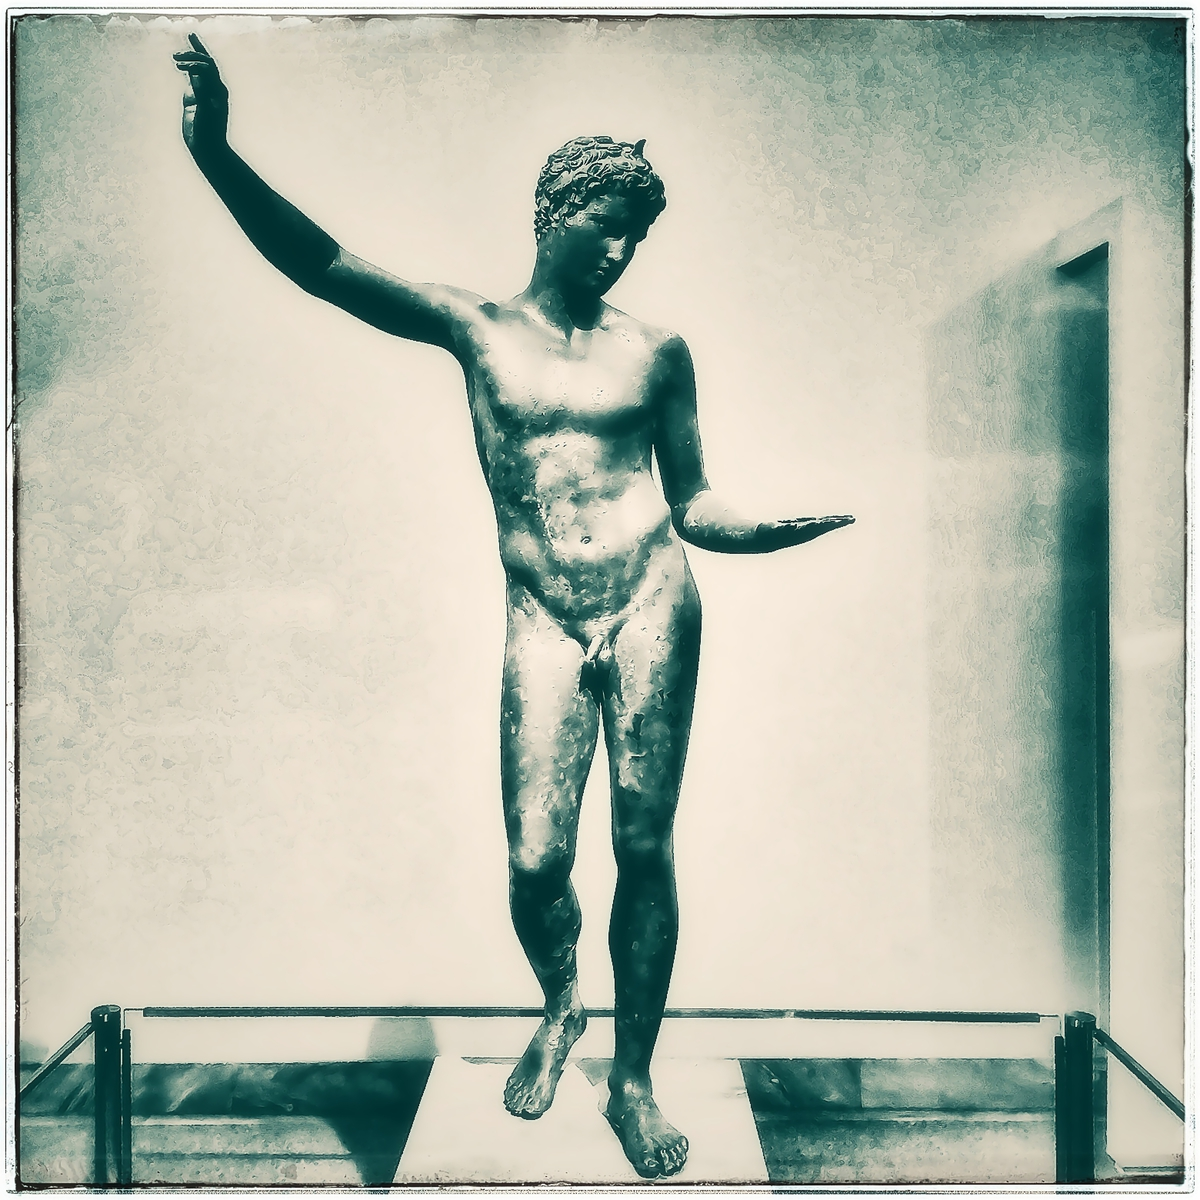
\includegraphics[width=0.72\linewidth]{thumb-lesson_IV.jpeg}
  \caption{Museo Nazionale di Archeologia di Atene}
  \label{fig:textfig}
  %\zsavepos{pos:textfig}
  \setfloatalignment{b}
\end{figure}

\nobibliography{greekBiblio}
\bibliographystyle{alpha}


\end{document}
